% Preamble
\documentclass[11pt]{article}

% Packages
\usepackage{amsmath}
\usepackage[italian]{babel}
\usepackage{graphics}
\usepackage{graphicx}
\usepackage{float}
\usepackage{csvsimple}
\usepackage{hyperref}
\usepackage{listings}
\usepackage{xcolor}
\usepackage{subcaption}
\usepackage{mdwtab}

\definecolor{codegreen}{rgb}{0,0.6,0}
\definecolor{codegray}{rgb}{0.5,0.5,0.5}
\definecolor{codepurple}{rgb}{0.58,0,0.82}
\definecolor{backcolour}{rgb}{0.95,0.95,0.92}

\lstdefinestyle{mystyle}{
    backgroundcolor=\color{backcolour},
    commentstyle=\color{codegreen},
    keywordstyle=\color{magenta},
    numberstyle=\tiny\color{codegray},
    stringstyle=\color{codepurple},
    basicstyle=\ttfamily\footnotesize,
    breakatwhitespace=false,
    breaklines=true,
    captionpos=b,
    keepspaces=true,
    numbers=left,
    numbersep=5pt,
    showspaces=false,
    showstringspaces=false,
    showtabs=false,
    tabsize=2
}
\lstset{style=mystyle}
\graphicspath{{../results/}}

% Document
\title{Problemi di Render : Parallel Programming for Machine Learning}
\author{Lorenzo Baiardi, Thomas Del Moro}
\date{10 12 2023}

\begin{document}

    \maketitle
    \clearpage

    \section{Introduzione}\label{sec:introduzione}
    In questo elaborato verificheremo l'efficacia dell'utilizzo di vari metodi di parallelizzazione in problemi comuni,
    studiandone i tempi di esecuzione.
    In particolare valutiamo il metodo del compositing tra piani tramite l'utilizzo della libreria grafica OpenCV\@.

    \section{Analisi del problema}\label{sec:analisi-del-problema}
    Ogni piano ha 4 canali di colore (RGBA) e per ogni piano verranno disegnati n cerchi in maniera del tutto casuale.
    Durante la fase di compositing dei piani, verrà applicato un effetto di trasparenza in base alla posizione del piano
    all'interno della sommatoria, in modo da ottenere un effetto di profondità.
    L'immagine risultante sarà salvata come file PNG\@ e metterà in risalto principalmente il piano, quindi cerchi,
    più in alto.

    \begin{figure}[h!]
        \begin{minipage}{0.32\textwidth}
            \centering
            
\includegraphics[width=\textwidth]{img/seq/10000}
            \caption{Sequenziale}
        \end{minipage}%
        \hfill
        \begin{minipage}{0.32\textwidth}
            \centering
            
\includegraphics[width=\textwidth]{img/par/10000}
            \caption{OMP}
        \end{minipage}%
        \hfill
        \begin{minipage}{0.32\textwidth}
            \centering
            
\includegraphics[width=\textwidth]{img/cuda/10000}
            \caption{CUDA}
        \end{minipage}
        \caption{Immagini di esempio}\label{fig:example-images}
    \end{figure}

    \section{Metodi di parallelizzazione}\label{sec:metodi-di-parallelizazzione}
    Per poter parallelizzare il problema abbiamo deciso di utilizzare due approcci differenti, nel primo caso abbiamo
    utilizzato la libreria OPENMP, al variare del numero di thread, e nel secondo caso abbiamo utilizzato il linguaggio
    di programmazione CUDA per il calcolo parallelo su scheda grafica\@.
    \lstinputlisting[language=c++, firstline=38, lastline=62,label={lst:sequential-code}]{../src/renderer.cu}

    \subsection{OPENMP}\label{subsec:openmp}
    L'idea di fondo è quella che ogni thread gestisca la sommatoria di un singolo pixel per ogni matrice, in
    modo da preservare l'ordinamento dei piani ma aumentandone la velocità di render.
    Di conseguenza ogni thread calcolerà il pixel risultante e successivamente, al termine di esso, passerà
    al successivo pixel.
    \lstinputlisting[language=c++, firstline=64, lastline=89,label={lst:parallel-code}]{../src/renderer.cu}


    \subsection{CUDA}\label{subsec:cuda}
    In questo caso la parte di parallelizzazione si svilupperà principalmente nel calcolo di grid e block da utilizzare,
    in modo da poter sfruttare al meglio la potenza di calcolo della scheda grafica.
    \lstinputlisting[language=c++, firstline=136, lastline=160,label={lst:cuda-code}]{../src/renderer.cu}

    \section{Caratteristiche della macchina}\label{sec:caratteristiche-della-macchina}
    La macchina utilizzata per effettuare i test è dotata di:
    \begin{itemize}
        \item Processore Intel Core i5-8600K 3.60 GHz (6 core)
        \item 16 GB di RAM
        \item Scheda grafica NVIDIA GeForce GTX 1050 Ti 4 GB
        \item Sistema operativo Windows 11
    \end{itemize}

    \section{Tests}\label{sec:tests}
    I test sono stati quindi effettuati al variare del numero dei piani e dalle dimensioni delle immagini.
    Tutti i piani e i vari cerchi vengono generati precedentemente all'esecuzione del test, in modo da poter avere
    un confronto più accurato tra i vari metodi di parallelizzazione.
    Le dimensioni delle immagini utilizzate sono 256x256, 512x512 e 1024x1024.
    Il numero di piani partono da 1000 e arrivano a 10000, con un incremento di 1000 piani per i test 256x256 e 512x512,
    mentre per il test 1024x1024 il numero di piani parte da 100 e arriva a 1000, con un incremento di 100 piani.
    Per la sola versione OpenMP è stata utilizzata la toolchain di MinGW, mentre per la versione CUDA è stata utilizzata
    la toolchain di MSVC\@.
    La versione di OpenCV utilizzata è la 4.6.0, mentre la versione di CUDA è la 11.8.

    \subsection{256x256}\label{subsec:256x256}
    \begin{figure}[H]
        \centering
        \begin{minipage}{0.49\textwidth}
            \centering
            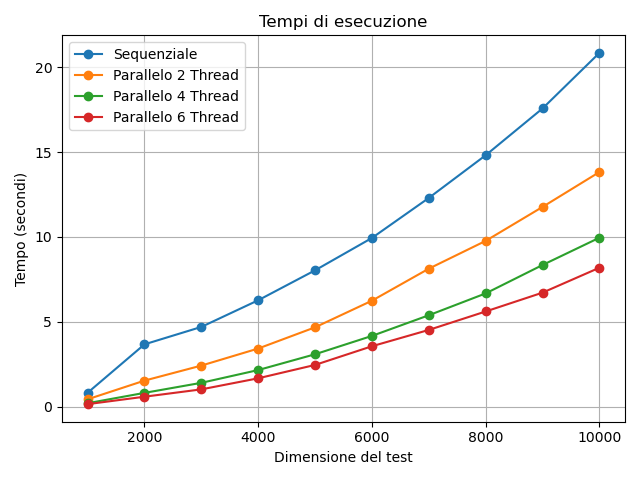
\includegraphics[width=\textwidth]{plots/256/omp_times}
            \caption{Tempi di OMP}\label{fig:times-256-omp}
        \end{minipage}
        \begin{minipage}{0.49\textwidth}
            \centering
            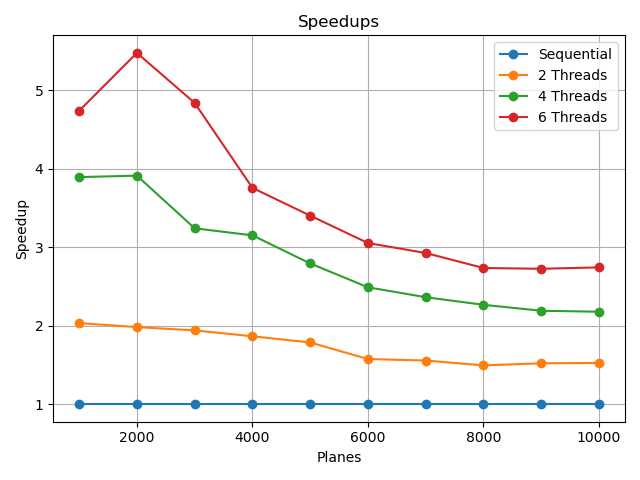
\includegraphics[width=\textwidth]{plots/256/omp_speedup}
            \caption{Speedup di OMP}\label{fig:speedup-256-omp}
        \end{minipage}
    \end{figure}

    \begin{figure}[H]
        \centering
        \begin{minipage}{0.49\textwidth}
            \centering
            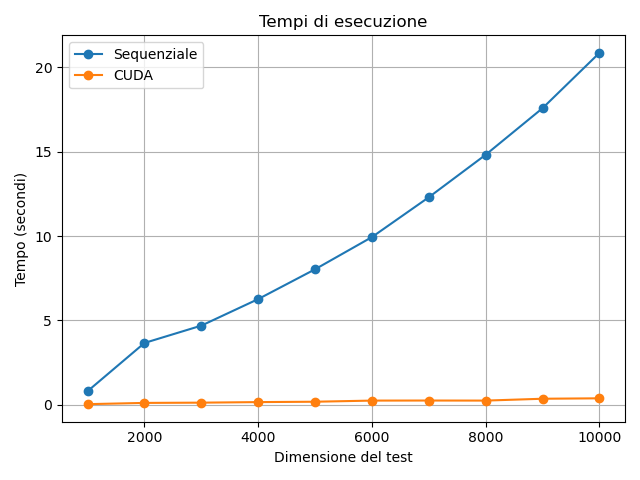
\includegraphics[width=\textwidth]{plots/256/cuda_times}
            \caption{Tempi di CUDA}\label{fig:times-256-cuda}
        \end{minipage}
        \begin{minipage}{0.49\textwidth}
            \centering
            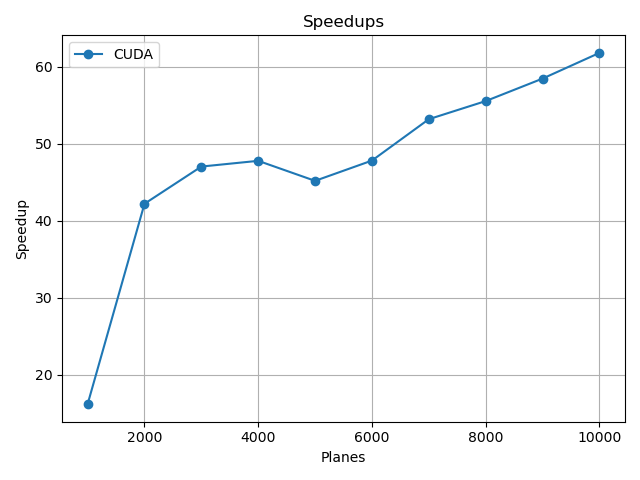
\includegraphics[width=\textwidth]{plots/256/cuda_speedup}
            \caption{Speedup di CUDA}\label{fig:speedup-256-cuda}
        \end{minipage}
    \end{figure}

    \begin{figure}[H]
        \centering
        \begin{minipage}{0.49\textwidth}
            \centering
            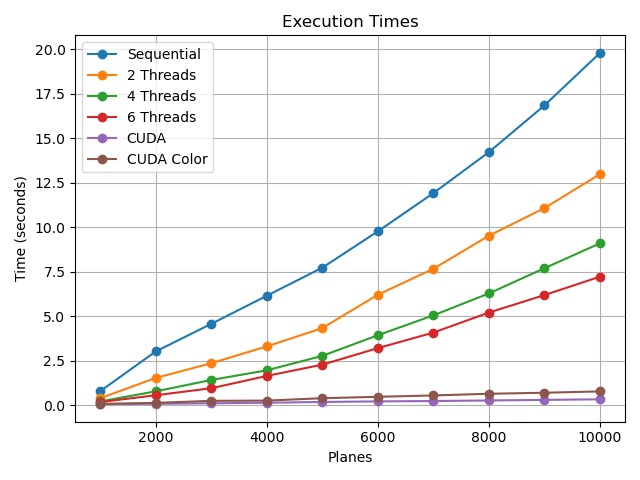
\includegraphics[width=\textwidth]{plots/256/results_times}
            \caption{Confronto dei tempi}\label{fig:tempi-256}
        \end{minipage}
        \begin{minipage}{0.49\textwidth}
            \centering
            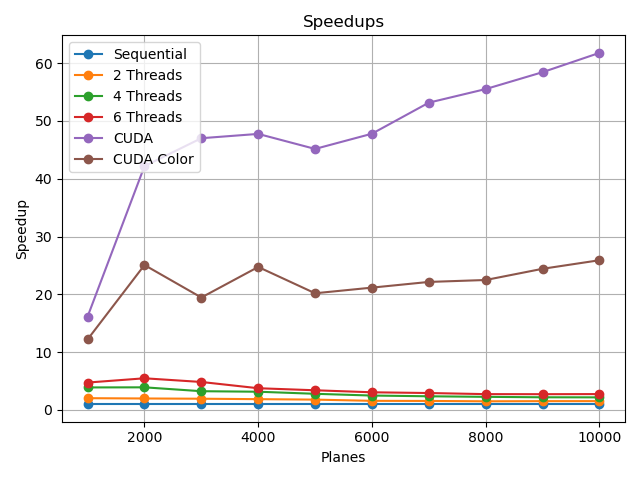
\includegraphics[width=\textwidth]{plots/256/results_speedup}
            \caption{Confronto fra speedups}\label{fig:speedups-256}
        \end{minipage}
    \end{figure}

    \subsection{512x512}\label{subsec:512x512}
    \begin{figure}[H]
        \centering
        \begin{minipage}{0.49\textwidth}
            \centering
            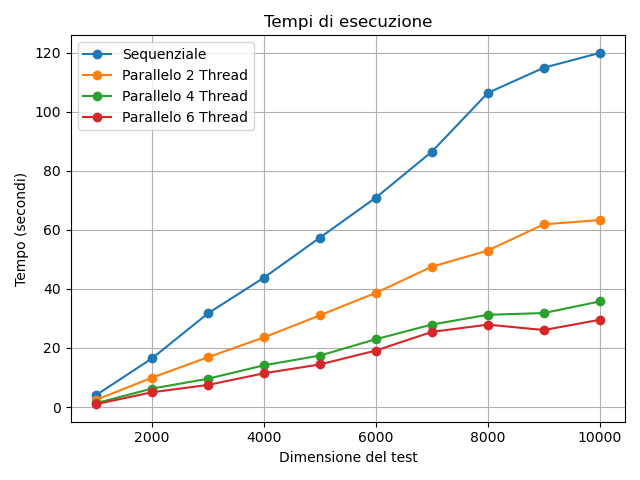
\includegraphics[width=\textwidth]{plots/512/omp_times}
            \caption{Tempi di OMP}\label{fig:times-512-omp}
        \end{minipage}
        \begin{minipage}{0.49\textwidth}
            \centering
            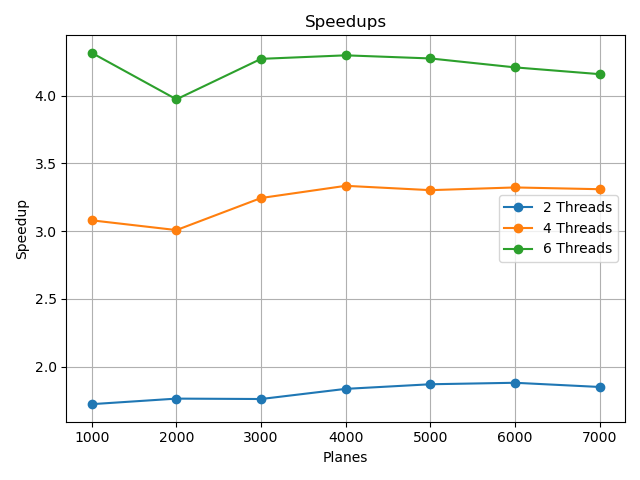
\includegraphics[width=\textwidth]{plots/512/omp_speedup}
            \caption{Speedup di OMP}\label{fig:speedup-512-omp}
        \end{minipage}
    \end{figure}

    \begin{figure}[H]
        \centering
        \begin{minipage}{0.49\textwidth}
            \centering
            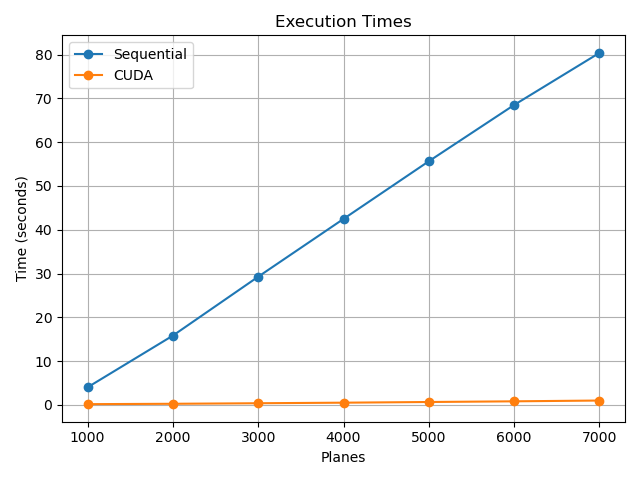
\includegraphics[width=\textwidth]{plots/512/cuda_times}
            \caption{Tempi di CUDA}\label{fig:times-512-cuda}
        \end{minipage}
        \begin{minipage}{0.49\textwidth}
            \centering
            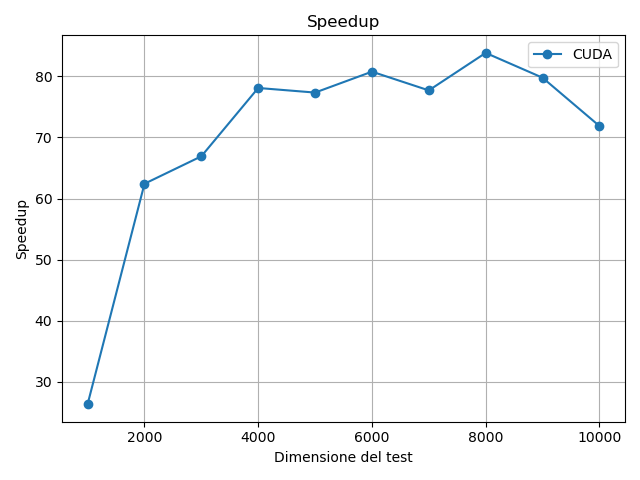
\includegraphics[width=\textwidth]{plots/512/cuda_speedup}
            \caption{Speedup di CUDA}\label{fig:speedup-512-cuda}
        \end{minipage}
    \end{figure}

    \begin{figure}[H]
        \centering
        \begin{minipage}{0.49\textwidth}
            \centering
            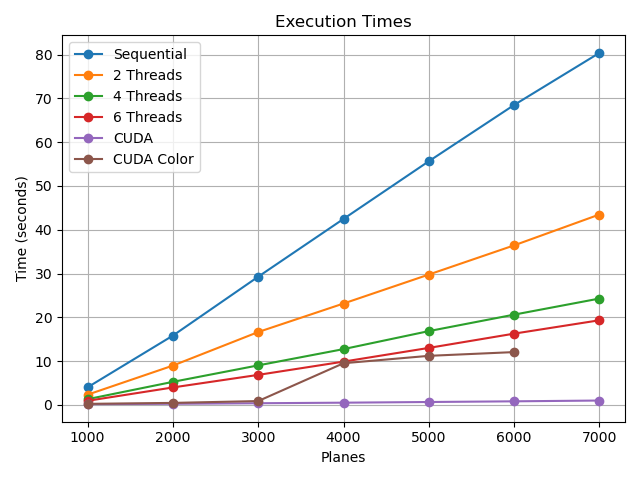
\includegraphics[width=\textwidth]{plots/512/results_times}
            \caption{Confronto dei tempi}\label{fig:tempi-512}
        \end{minipage}
        \begin{minipage}{0.49\textwidth}
            \centering
            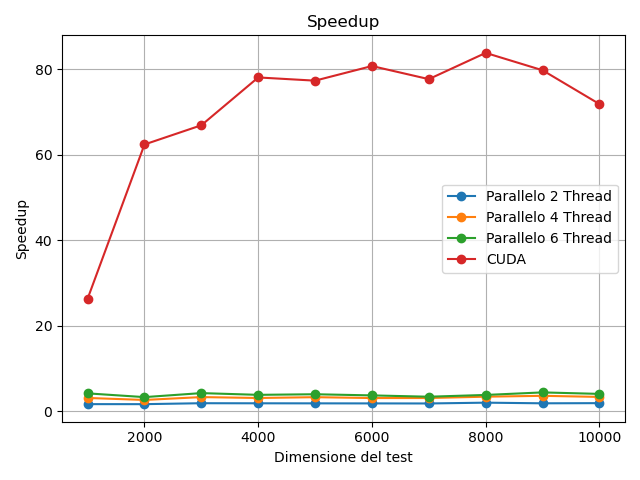
\includegraphics[width=\textwidth]{plots/512/results_speedup}
            \caption{Confronto fra speedups}\label{fig:speedups-512}
        \end{minipage}
    \end{figure}

    \subsection{1024x1024}\label{subsec:1024x1024}
    \begin{figure}[H]
        \centering
        \begin{minipage}{0.49\textwidth}
            \centering
            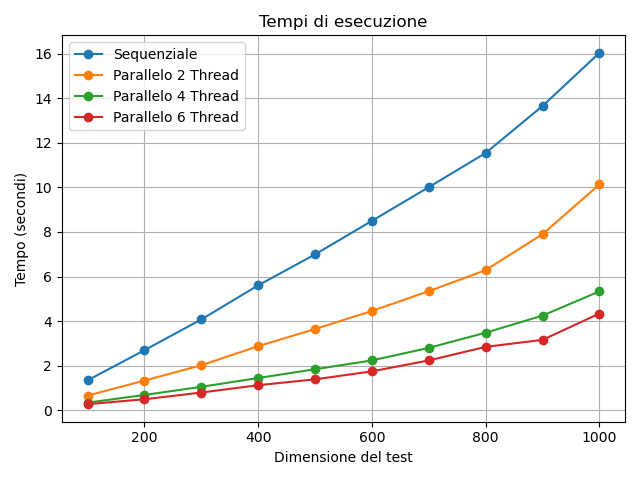
\includegraphics[width=\textwidth]{plots/1024/omp_times}
            \caption{Tempi di OMP}\label{fig:times-1024-omp}
        \end{minipage}
        \begin{minipage}{0.49\textwidth}
            \centering
            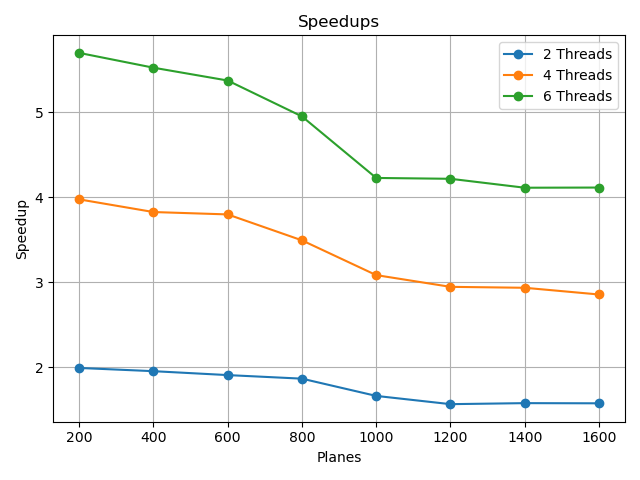
\includegraphics[width=\textwidth]{plots/1024/omp_speedup}
            \caption{Speedup di OMP}\label{fig:speedup-1024-omp}
        \end{minipage}
    \end{figure}

    \begin{figure}[H]
        \centering
        \begin{minipage}{0.49\textwidth}
            \centering
            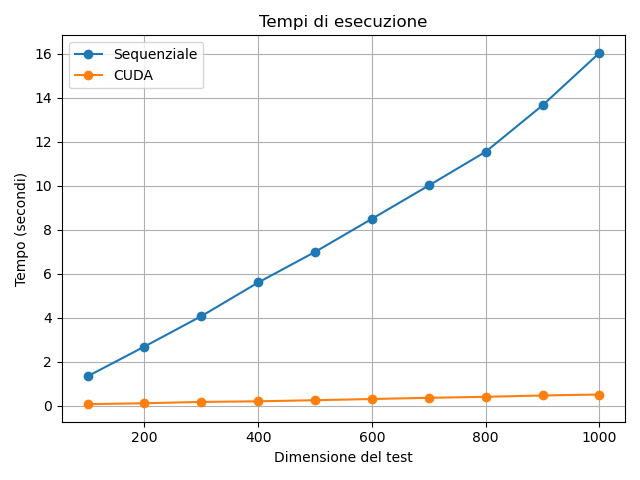
\includegraphics[width=\textwidth]{plots/1024/cuda_times}
            \caption{Tempi di CUDA}\label{fig:times-1024-cuda}
        \end{minipage}
        \begin{minipage}{0.49\textwidth}
            \centering
            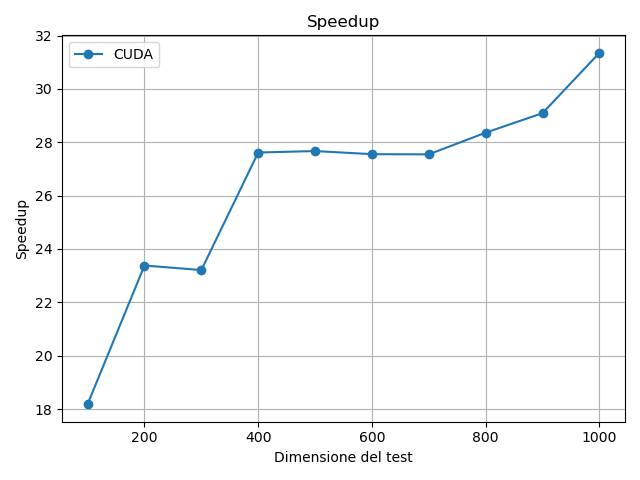
\includegraphics[width=\textwidth]{plots/1024/cuda_speedup}
            \caption{Speedup di CUDA}\label{fig:speedup-1024-cuda}
        \end{minipage}
    \end{figure}

    \begin{figure}[H]
        \centering
        \begin{minipage}{0.49\textwidth}
            \centering
            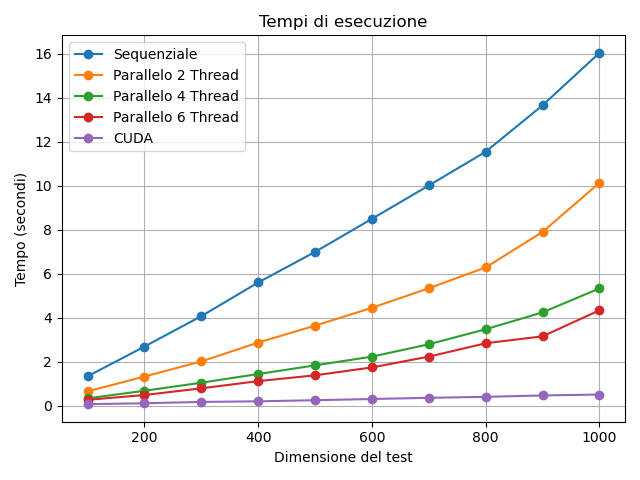
\includegraphics[width=\textwidth]{plots/1024/results_times}
            \caption{Confronto dei tempi}\label{fig:tempi-1024}
        \end{minipage}
        \begin{minipage}{0.49\textwidth}
            \centering
            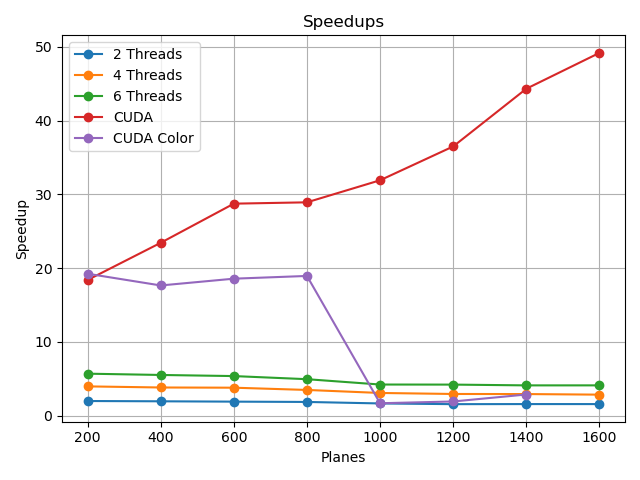
\includegraphics[width=\textwidth]{plots/1024/results_speedup}
            \caption{Confronto fra speedups}\label{fig:speedups-1024}
        \end{minipage}
    \end{figure}

    \section{Conclusioni}\label{sec:conclusioni}
    In conclusione, come è possibile vedere dai vari test effettuati e come ci si potesse aspettare, l'operazione di
    parallelizzazione CUDA risulti quello che ottiene un maggior incremento a livello di speedUp nei vari test
    effettuati.
    Questo è dovuto principalmente al fatto che la scheda grafica è stata progettata per effettuare operazioni
    parallele, quindi è possibile sfruttare al meglio la potenza di calcolo della scheda grafica.
    Inoltre, come è possibile vedere dai vari test effettuati, l'incremento di velocità è maggiore al crescere del
    numero di piani, questo è dovuto al fatto che la scheda grafica riesce a sfruttare al meglio la sua potenza di
    calcolo al crescere del numero di piani.
    E' da notare anche come la versione parallela di OpenMP riesca a ottenere un incremento di velocità maggiore
    rispetto alla versione sequenziale, specialmente all'aumentare del numero di thread che la macchina dispone.

    \clearpage

    \section{Risultati}\label{sec:risultati}
    \begin{table}[!ht]
        \centering
        \begin{subtable}{0.45\textwidth}
            \centering
            \begin{tabular}{|c|c|c|c|}
                \hline
                Test & TSeq & TPar & SpeedUp \\ \hline
                1000 & 4.031 & 2.423 & 1.664 \\ \hline
                2000 & 16.495 & 9.949 & 1.658 \\ \hline
                3000 & 31.754 & 16.896 & 1.879 \\ \hline
                4000 & 43.843 & 23.582 & 1.859 \\ \hline
                5000 & 57.414 & 31.088 & 1.847 \\ \hline
                6000 & 70.984 & 38.698 & 1.834 \\ \hline
                7000 & 86.536 & 47.558 & 1.820 \\ \hline
                8000 & 106.463 & 53.034 & 2.007 \\ \hline
                9000 & 114.997 & 61.922 & 1.857 \\ \hline
                10000 & 120.016 & 63.340 & 1.895 \\ \hline
            \end{tabular}
            \caption{Risultati parallelo 2}\label{tab:table-parallel2}
        \end{subtable}
        \hfill
        \begin{subtable}{0.45\textwidth}
            \centering
            \begin{tabular}{|c|c|c|c|}
                \hline
                Test & TSeq & TPar & SpeedUp \\ \hline
                1000 & 4.031 & 1.297 & 3.109 \\ \hline
                2000 & 16.495 & 6.244 & 2.642 \\ \hline
                3000 & 31.754 & 9.585 & 3.313 \\ \hline
                4000 & 43.843 & 14.141 & 3.100 \\ \hline
                5000 & 57.414 & 17.439 & 3.292 \\ \hline
                6000 & 70.984 & 22.983 & 3.089 \\ \hline
                7000 & 86.536 & 27.962 & 3.095 \\ \hline
                8000 & 106.463 & 31.255 & 3.406 \\ \hline
                9000 & 114.997 & 31.843 & 3.611 \\ \hline
                10000 & 120.016 & 35.780 & 3.354 \\ \hline
            \end{tabular}
            \caption{Risultati parallelo 4}\label{tab:table-parallel4}
        \end{subtable}


        \centering
        \begin{subtable}{0.45\textwidth}
            \centering
            \begin{tabular}{|c|c|c|c|}
                \hline
                Test & TSeq & TPar & SpeedUp \\ \hline
                1000 & 4.031 & 0.964 & 4.182 \\ \hline
                2000 & 16.495 & 4.991 & 3.305 \\ \hline
                3000 & 31.754 & 7.483 & 4.244 \\ \hline
                4000 & 43.843 & 11.426 & 3.837 \\ \hline
                5000 & 57.414 & 14.432 & 3.978 \\ \hline
                6000 & 70.984 & 19.149 & 3.707 \\ \hline
                7000 & 86.536 & 25.457 & 3.399 \\ \hline
                8000 & 106.463 & 27.917 & 3.814 \\ \hline
                9000 & 114.997 & 26.086 & 4.408 \\ \hline
                10000 & 120.016 & 29.564 & 4.060 \\ \hline
            \end{tabular}
            \caption{Risultati parallelo 6}\label{tab:table-parallel6}
        \end{subtable}
        \hfill
        \begin{subtable}{0.45\textwidth}
            \centering
            \begin{tabular}{|c|c|c|c|}
                \hline
                Test & TSeq & TCuda & SpeedUp \\ \hline
                1000 & 4.031 & 0.153 & 26.329 \\ \hline
                2000 & 16.495 & 0.264 & 62.419 \\ \hline
                3000 & 31.754 & 0.475 & 66.915 \\ \hline
                4000 & 43.843 & 0.561 & 78.102 \\ \hline
                5000 & 57.414 & 0.742 & 77.349 \\ \hline
                6000 & 70.984 & 0.879 & 80.771 \\ \hline
                7000 & 86.536 & 1.114 & 77.706 \\ \hline
                8000 & 106.463 & 1.270 & 83.846 \\ \hline
                9000 & 114.997 & 1.441 & 79.783 \\ \hline
                10000 & 120.016 & 1.670 & 71.877 \\ \hline
            \end{tabular}
            \caption{Risultati CUDA}\label{tab:table-cuda}
        \end{subtable}
        \caption{Confronto tra i risultati di parallelismo}\label{tab:table-comparison}
    \end{table}

\end{document}